\documentclass[12pt]{report}
\usepackage{polyglossia}
\setmainlanguage{vietnamese}
\usepackage{graphicx}
\graphicspath{{images/}}
\usepackage[a4paper]{geometry}
\usepackage{lipsum}
\usepackage{fancyhdr}
\usepackage{indentfirst}
% \setlength{\parindent}{15pt}
\pagestyle{fancy}
\fancyhead{}
\fancyhead[L]{\leftmark}
% \fancyfoot{}
% \fancyfoot[R]{\thepage}
% \fancyfoot[L]{Chương \thechapter}
% \fancyfoot[C]{Bùi Minh Thắng}
\fancyheadoffset[R]{0mm}
\usepackage{fontspec}
\setmainfont{Times New Roman}
\usepackage{tikz}
\usetikzlibrary{calc}
\usepackage{listings}
\usepackage{xcolor}
\usepackage{courier}
\usepackage{amsmath}
\usepackage{amssymb}
\usepackage{float}
\usepackage{biblatex}
\addbibresource{refs.bib}

\title{
    {Thesis Title}\\
    {\large Institution Name}\\
    % {\includegraphics{UET_logo.png}}
}
\author{Bùi Minh Thắng}
\date{March 2025}

\begin{document}
% \fontsize{14pt}{18pt}\selectfont

\newgeometry{
    top=2.2cm,
    bottom=2.2cm,
    left=2.2cm,
    right=2.2cm
}

\begin{titlepage}
    \begin{tikzpicture}[overlay,remember picture]
    \draw [line width=0.5mm]
        ($ (current page.north west) + (2cm,-2cm) $)
        rectangle
        ($ (current page.south east) + (-2cm,2cm) $);
    \draw [line width=0.5m  m]
        ($ (current page.north west) + (1.9cm,-1.9cm) $)
        rectangle
        ($ (current page.south east) + (-1.9cm,1.9cm) $);
    \end{tikzpicture}
    \begin{center}
        \large\textbf{ĐẠI HỌC QUỐC GIA HÀ NỘI}\\
        \large\textbf{TRƯỜNG ĐẠI HỌC CÔNG NGHỆ}\\
        ----------------***---------------

        \vspace{3cm}
        {\large\textbf{BÁO CÁO THU HOẠCH HỌC PHẦN CÁC VẤN ĐỀ HIỆN ĐẠI CỦA TRUYỀN THÔNG VÀ MẠNG MÁY TÍNH}}

        \vspace{3cm}
        {\huge\textbf{Các Khía Cạnh Điều Khiển trong Hệ Thống MEC Hỗ Trợ bởi RIS cho Ứng Dụng Độ Trễ Nghiêm Ngặt}}

        \vfill
        \begin{table}[h]
            \centering
            \large
            \begin{tabular}{ll}
                \textbf{Họ và Tên:} & Bùi Minh Thắng - 23020646 \\
                \textbf{          } & Nguyễn Vũ Minh - 23020629 \\
                \textbf{          } & Ma Đức Minh - 23020626 \\
                \textbf{          } & Nguyễn Hoàng Tùng Dương - 21020182 \\
                \textbf{Người hướng dẫn:} & TS. Nguyễn Ngọc Tân \\
                \textbf{                } & CN. Nguyễn Thái Dương \\
            \end{tabular}
        \end{table}

        \vspace{4cm}
        \textbf{Hà Nội, 2025}
        
    \end{center}
\end{titlepage}

\newgeometry{
    top=2cm,
    bottom=2cm,
    left=3cm,
    right=2cm
}

\chapter*{Lời cam đoan}
Nhóm em xin cam đoan: Báo cáo nghiên cứu khoa học với đề tài “Các Khía Cạnh Điều Khiển trong Hệ Thống MEC Hỗ Trợ bởi RIS cho Ứng Dụng Độ Trễ Nghiêm Ngặt” này là của nhóm em. Những gì nhóm em viết ra không có sự sao chép từ các tài liệu, không sử dụng kết quả của người khác mà không trích dẫn cụ thể. Đây là công trình nghiên cứu tập thể nhóm em tự phát triển, không sao chép mã nguồn của người khác. Nếu vi phạm những điều trên, nhóm em xin chấp nhận tất cả những truy cứu về trách nhiệm theo quy định.

\vspace{2cm} % nếu cần tạo khoảng cách từ nội dung phía trên
\noindent
\hfill
\begin{minipage}{0.4\textwidth}
    \centering
    \textbf{Sinh viên}\\[1cm] % khoảng trống cho chữ ký
    Bùi Minh Thắng\\
    Nguyễn Vũ Minh\\
    Ma Đức Minh\\
    Nguyễn Hoàng Tùng Dương\\
\end{minipage}

\chapter*{Lời cảm ơn}
Lời đầu tiên, em xin được gửi lời cảm ơn chân thành tới Khoa Công nghệ Thông tin – Trường Đại học Công nghệ – Đại học Quốc gia Hà Nội đã tạo điều kiện thuận lợi để em được học tập, nghiên cứu và thực hiện đề tài này.

Em xin bày tỏ lòng biết ơn sâu sắc tới thầy Nguyễn Ngọc Tân và thầy Nguyễn Thái Dương đã tận tình hướng dẫn, hỗ trợ em trong suốt quá trình nghiên cứu và triển khai đề tài.

Bên cạnh đó, em xin được bày tỏ lòng biết ơn tới các thầy cô trong khoa đã tận tâm giảng dạy và trang bị cho em những kiến thức quý báu trong suốt quá trình học tập tại trường.

Cuối cùng, em xin chúc các thầy cô, các bạn luôn mạnh khỏe, hạnh phúc và gặt hái nhiều thành công trong cuộc sống.

\chapter*{Tóm tắt}
Hệ thống tính toán biên di động (Mobile Edge Computing - MEC) kết hợp với các bề mặt thông minh có thể tái cấu hình (Reconfigurable Intelligent Surfaces - RIS) nổi lên như một giải pháp tiềm năng để đáp ứng yêu cầu độ trễ cực thấp của các ứng dụng tương lai (như IoT, điều khiển công nghiệp, xe tự hành). Báo cáo này tập trung phân tích các khía cạnh điều khiển – bao gồm việc ước lượng kênh (CE), phân bổ tài nguyên (RA) và tín hiệu điều khiển – trong hệ thống MEC có hỗ trợ RIS, đặc biệt nhấn mạnh vai trò của overhead điều khiển đối với hiệu năng và độ trễ end-to-end. Trong các hệ thống này, việc đầu tư nhiều tài nguyên cho điều khiển sẽ nâng cao độ tin cậy (ví dụ ước lượng kênh chính xác hơn, phân bổ tài nguyên tối ưu hơn), nhưng đồng thời giảm quỹ thời gian và tài nguyên dành cho truyền dữ liệu, có thể tăng độ trễ tổng thể. Ngược lại, giảm overhead điều khiển giúp dành nhiều thời gian hơn để offload dữ liệu, nhưng có thể làm giảm chất lượng CSI và độ linh hoạt trong RA
. Báo cáo xây dựng một khung phân tích tác động của các tác vụ điều khiển này đến hiệu năng hệ thống MEC/RIS, làm rõ sự đánh đổi giữa hiệu năng và độ trễ thông qua phân tích lý thuyết và kết quả mô phỏng từ bài báo gốc \cite{ris_latency}. Các yếu tố như thời gian overhead, chi phí năng lượng cho điều khiển, và ảnh hưởng của lỗi điều khiển (do kênh điều khiển không hoàn hảo) được xem xét sâu sắc. Ngoài ra, báo cáo so sánh giữa RIS thụ động vs. RIS chủ động trong bối cảnh MEC: RIS chủ động có thể cải thiện hiệu năng nhờ khuếch đại tín hiệu nhưng đòi hỏi năng lượng và phức tạp cao hơn, trong khi RIS thụ động tiết kiệm năng lượng nhưng chịu suy hao kênh kép lớn. Cuối cùng, chúng tôi tổng hợp các hướng nghiên cứu mới nhằm giảm overhead điều khiển (như thuật toán ước lượng kênh hiệu quả, phân bổ tài nguyên bền vững với lỗi, điều khiển hai thang thời gian, v.v.) và đề xuất một số cải tiến tương lai để tối ưu hóa hơn nữa sự tích hợp RIS trong MEC cho các ứng dụng có độ trễ nghiêm ngặt.

\textbf{Từ khoá:} MEC, RIS, tính toán biên di động, độ trễ đầu-cuối, điều khiển kênh, overhead điều khiển, ước lượng kênh (CE), phân bổ tài nguyên (RA), RIS chủ động, RIS thụ động.

\tableofcontents

% % \listoffigures

% % \listoftables

% % \chapter*{Thuật ngữ}


\chapter{Giới thiệu}
Trong những năm gần đây, sự phát triển bùng nổ của các dịch vụ viễn thông, đặc biệt là các ứng dụng yêu cầu tốc độ cao, độ trễ thấp và khả năng quản lý linh hoạt, đã đặt ra những thách thức mới đối với hạ tầng mạng truyền thống. Kiến trúc mạng truy cập vô tuyến truyền thống (RAN) với các thiết bị và giao diện đóng độc quyền gây ra nhiều hạn chế về tính linh hoạt, khả năng tương tác và đổi mới công nghệ. Chính vì vậy, xu hướng chuyển dịch sang kiến trúc mạng truy cập vô tuyến mở (Open RAN) ngày càng thu hút sự quan tâm lớn từ cộng đồng nghiên cứu và các nhà cung cấp dịch vụ viễn thông hàng đầu thế giới.

Open RAN được kỳ vọng sẽ tái định hình ngành công nghiệp viễn thông nhờ vào việc mở các giao diện, phân tách chức năng mạng (như Central Unit - CU, Distributed Unit - DU, và Radio Unit - RU), đồng thời đưa trí tuệ nhân tạo (AI) vào sâu hơn trong việc quản lý và vận hành mạng lưới. Một thành phần cốt lõi giúp đạt được những lợi ích này chính là bộ điều khiển thông minh mạng vô tuyến (RAN Intelligent Controller - RIC) với hai phiên bản chính là Near-Real-Time RIC và Non-Real-Time RIC. Hai loại RIC này giúp quản lý và tối ưu các ứng dụng mạng (xApps và rApps) trong thời gian thực hoặc gần thực.

Mục tiêu của báo cáo này là làm rõ những ưu điểm của Open RAN so với mạng RAN truyền thống, đồng thời phân tích cụ thể vai trò của các thành phần quan trọng như RIC và các giao diện mở (E2, A1, O1). Qua đó, nhóm nghiên cứu mong muốn đề xuất một mô hình tối ưu hóa tài nguyên mạng hiệu quả bằng công nghệ học tăng cường sâu (DRL) nhằm đáp ứng các yêu cầu về hiệu năng, linh hoạt và khả năng mở rộng của mạng viễn thông thế hệ mới.

\chapter{Tổng quan về MEC và RIS trong mạng 5G/6G}
\section{Mobile Edge Computing (MEC) – Tính toán biên di động}


MEC là một kiến trúc tính toán phân tán, trong đó tài nguyên xử lý và lưu trữ đám mây được bố trí tại biên mạng di động, gần với phía người dùng hơn so với đám mây truyền thống. Ý tưởng chính của MEC là giảm khoảng cách vật lý giữa thiết bị người dùng (UE) và máy chủ thực thi tác vụ, qua đó giảm độ trễ truyền dẫn và tiết kiệm băng thông backhaul \cite{ris_latency}. Trong MEC, các UE có thể offload (tải lên) một phần hoặc toàn bộ tác vụ tính toán nặng (ví dụ: xử lý ảnh, video, phân tích dữ liệu IoT, AI...) đến máy chủ MEC đặt tại các trạm gốc hoặc điểm truy cập WiFi cục bộ. Máy chủ MEC, tuy có năng lực hạn chế hơn cloud trung tâm, nhưng nhờ vị trí gần UE nên có thể trả kết quả nhanh, đáp ứng yêu cầu độ trễ nghiêm ngặt của ứng dụng thời gian thực. 


Có hai chế độ offload phổ biến: (i) Offload toàn phần (binary offloading) – toàn bộ tác vụ được gửi lên MEC hoặc xử lý cục bộ, phù hợp với tác vụ nhỏ, không thể tách; (ii) Offload từng phần (partial offloading) – tác vụ được chia thành nhiều phần, một phần xử lý tại UE, phần còn lại gửi lên MEC, phù hợp với tác vụ lớn có thể song song hóa \cite{ris_latency}. MEC đã chứng minh hiệu quả trong giảm trễ so với điện toán đám mây truyền thống, nhưng vẫn gặp thách thức khi kênh vô tuyến không đảm bảo hoặc số lượng thiết bị lớn. Để nâng cao thông lượng offload, nhiều giải pháp bổ trợ đã được nghiên cứu: mạng di động không đồng nhất (HetNet) với các small-cell để giảm khoảng cách UE-AP; sử dụng massive MIMO tại trạm gốc để tăng phân tập và chống nhiễu; truyền ở băng tần mmWave hay THz để có băng thông rộng hơn cho offload; dùng UAV làm trạm di động để tạo đường truyền LOS linh hoạt. Tuy nhiên, các giải pháp này cũng có nhược điểm riêng (chi phí triển khai cao, kiến trúc phức tạp, tiêu thụ năng lượng lớn). Do đó, xuất hiện nhu cầu tìm kiếm giải pháp khác bổ trợ MEC hiệu quả, đặc biệt trong bối cảnh 6G.
\section{Chức năng của Near-Real-Time RIC và Non-Real-Time RIC}
Trong kiến trúc mạng truy cập vô tuyến mở (Open RAN), Bộ điều khiển RAN thông minh (RAN Intelligent Controller – RIC) được phân tách thành hai phần: RIC thời gian gần thực (Near-Real-Time RIC) và RIC thời gian không thực (Non-Real-Time RIC). Hai thành phần này phối hợp điều khiển và tối ưu mạng ở những quy mô thời gian khác nhau nhằm nâng cao hiệu năng của RAN. Cụ thể, Near-RT RIC đảm nhiệm việc điều khiển RAN với độ trễ thấp (từ khoảng 10 mili-giây đến <1 giây) \cite{Understanding_O-Ran}, còn Non-RT RIC phụ trách các tác vụ ở quy mô thời gian dài hơn (>1 giây, thường tính bằng giây, phút hoặc lâu hơn) \cite{Understanding_O-Ran}. Sự phân chia này cho phép tối ưu mạng ở cả thời gian thực ngắn hạn lẫn hoạch định dài hạn, tạo nên hệ thống điều khiển nhiều tầng cho RAN.

Near-Real-Time RIC (Near-RT RIC): Đây là thành phần RIC hoạt động gần thời gian thực, thường được triển khai trên hạ tầng điện toán biên hoặc cụm mạng khu vực gần với các nút RAN. Near-RT RIC có chức năng thu thập thông tin trạng thái mạng và thực thi các hành động điều khiển nhanh lên mạng vô tuyến với độ trễ yêu cầu dưới ~1 giây \cite{Understanding_O-Ran}. Theo đặc tả O-RAN, Near-RT RIC là một chức năng logic cho phép điều khiển và tối ưu tài nguyên RAN ở mức độ nhanh, thông qua việc thu thập dữ liệu chi tiết và tác động hành động lên các nút RAN qua giao diện E2 docs.o-ran-sc.org. Near-RT RIC thường xử lý các tác vụ như điều khiển truy cập vô tuyến và tài nguyên vô tuyến theo thời gian thực gần, ví dụ: điều phối lịch truyền dẫn, cân bằng tải giữa các cell, điều chỉnh tham số handover, điều khiển can nhiễu,… nhằm tối ưu hiệu suất thông lượng và chất lượng dịch vụ tức thời cho người dùng. Thành phần này tương tác trực tiếp với các nút mạng RAN (như O-DU, O-CU) qua giao diện E2 để nhận số liệu tình trạng (telemetry) và gửi chỉ thị điều khiển một cách liên tục. Đặc điểm quan trọng của Near-RT RIC là khả năng mở rộng chức năng qua các xApp – những ứng dụng plug-and-play chạy trên nền tảng Near-RT RIC để thực hiện các thuật toán điều khiển radio chuyên biệt \cite{Understanding_O-Ran}. Near-RT RIC cũng có cơ chế phối hợp và tránh xung đột giữa nhiều xApp khác nhau cùng tác động lên RAN (ví dụ: cơ chế quản lý message bus, lớp dữ liệu chia sẻ, và logic phân giải xung đột) để đảm bảo các quyết định điều khiển không mâu thuẫn \cite{Understanding_O-Ran}.

Non-Real-Time RIC (Non-RT RIC): Đây là thành phần RIC hoạt động ngoài thời gian thực chặt chẽ, nằm trong khối dịch vụ quản lý và điều hành (Service Management and Orchestration – SMO) ở trung tâm mạng hoặc đám mây. Non-RT RIC chịu trách nhiệm thực hiện các tác vụ quản lý, tối ưu RAN ở quy mô dài hạn hơn (trên 1 giây) \cite{Understanding_O-Ran}, bao gồm quản lý chính sách dịch vụ, phân tích hiệu năng, tối ưu cấu hình và hoạch định tài nguyên chiến lược cho mạng. Theo O-RAN Alliance, Non-RT RIC là một chức năng logic trong SMO hỗ trợ điều khiển/tối ưu RAN phi-thời-gian-thực, cung cấp khung AI/ML để huấn luyện và cập nhật mô hình, và truyền tải các hướng dẫn chính sách tới RIC gần thực \cite{Oran_overview} \cite{etsi_oranArchitecture}. Non-RT RIC được cấu thành bởi framework Non-RT RIC (nền tảng) và các ứng dụng rApp (các ứng dụng chạy trên Non-RT RIC). Nền tảng Non-RT RIC thực hiện việc kết thúc (terminate) giao diện A1 với Near-RT RIC, đồng thời phơi bày dịch vụ quản lý dữ liệu và ML cho các rApp thông qua giao diện nội bộ R1 \cite{etsi_oranArchitecture}. Các rApp (RAN applications) là những ứng dụng mô-đun chạy trên Non-RT RIC, sử dụng các dịch vụ mà nền tảng cung cấp để tạo ra các giá trị gia tăng cho vận hành RAN \cite{etsi_oranArchitecture}. Nhiệm vụ của rApp rất đa dạng, bao gồm: đề xuất và điều chỉnh chính sách điều khiển RAN, phân tích dữ liệu hiệu năng dài hạn, tối ưu cấu hình tham số, cũng như cung cấp thông tin bổ sung (enrichment information) cho các ứng dụng khác \cite{etsi_oranArchitecture}. Non-RT RIC gửi hướng dẫn chính sách và mục tiêu đến Near-RT RIC thông qua giao diện A1 (ví dụ: chính sách về phân bổ tài nguyên, mục tiêu QoS cần đạt, tham số ngưỡng sự kiện, v.v.), nhờ đó ảnh hưởng gián tiếp đến hành vi của các xApp trên Near-RT RIC \cite{etsi_oranArchitecture}. Ngược lại, Non-RT RIC cũng thu thập phản hồi từ mạng (thông qua dữ liệu O1 hoặc qua báo cáo từ Near-RT RIC) để đánh giá và điều chỉnh các chiến lược tối ưu. Có thể xem Non-RT RIC như “bộ não” ở tầng trên, vạch ra chiến lược dài hạn cho mạng, trong khi Near-RT RIC là “cánh tay tác động” ở tầng dưới thực thi các điều chỉnh nhanh theo chiến lược đó.
\section{Ứng dụng RIS trong MEC để giảm độ trễ}

Việc kết hợp RIS vào hệ thống MEC (tức RIS-aided MEC) được kỳ vọng nâng cao hiệu năng hệ thống trên nhiều phương diện. Thứ nhất, RIS giúp cải thiện chất lượng kênh truyền giữa UE và AP, từ đó tăng tốc độ offload dữ liệu từ UE lên edge server (ES)
\cite{ris_latency}
. Tốc độ offload cao cho phép UE gửi xong dữ liệu sớm hơn, ES xử lý sớm và trả kết quả sớm, nên giảm độ trễ tổng cho ứng dụng. Thứ hai, với sự hỗ trợ của RIS, MEC có thể phục vụ các UE ở vị trí trước đây sóng khó tới (góc khuất, vùng biên cell) mà vẫn đảm bảo băng thông, giúp mở rộng vùng phục vụ MEC mà không cần tăng công suất phát hay triển khai thêm trạm. Thứ ba, RIS có thể tiết kiệm năng lượng hệ thống: do kênh được cải thiện, UE có thể truyền ở công suất thấp hơn cho cùng lượng dữ liệu, hoặc ES không cần chờ nhiều lần truyền lại do lỗi, qua đó tổng năng lượng dùng để hoàn thành tác vụ giảm đi. 



Một ví dụ điển hình, công trình của P. Di Lorenzo và cs. (2022) đã nghiên cứu MEC động có RIS, trong đó UE liên tục sinh dữ liệu cần xử lý và kênh vô tuyến thay đổi theo thời gian. Kết quả cho thấy với RIS, có thể tối ưu hóa phối hợp cấu hình RIS, tham số truyền thông (phân bổ băng thông, công suất) và tài nguyên tính toán tại ES để đảm bảo độ trễ trung bình dưới ngưỡng trong khi tối thiểu hóa tiêu thụ năng lượng của toàn hệ (cả UE lẫn mạng)
\cite{mec}
. Tuy nhiên, tất cả các tối ưu kể trên giả định lý tưởng rằng thông tin kênh qua RIS và trạng thái hệ thống đều biết hoàn hảo và ngay lập tức. Như đã nêu, thực tế để đạt được điều đó cần các thủ tục điều khiển phức tạp. Phần tiếp theo, chúng tôi đi vào chi tiết mô hình hệ thống và các thủ tục này.
3. Mô hình hệ thống MEC h

% \chapter{Phương pháp tối ưu hoá ABR}
% \input{chapters/chapter03}

\chapter{Mô hình hệ thống MEC hỗ trợ RIS và các kênh điều khiển}
\section{Tổng quan về mô phỏng}

Nhằm minh họa rõ ràng và trực quan hóa các lợi ích từ việc ứng dụng kiến trúc Open RAN và điều khiển thông minh dựa trên học tăng cường sâu (DRL), nhóm đã quyết định lựa chọn công cụ mô phỏng mã nguồn mở RIMEDO-TS của dự án ONOS. RIMEDO-TS là bộ công cụ được phát triển nhằm mô phỏng và đánh giá hiệu suất các thuật toán quản lý tài nguyên và điều khiển thông minh trong môi trường Open RAN, đặc biệt nhấn mạnh vào khả năng tích hợp dễ dàng các xApp dựa trên AI và DRL.


\section{Giới thiệu về RIMEDO-TS}
RIMEDO-TS được phát triển bởi dự án ONOS (Open Network Operating System), cung cấp môi trường mô phỏng chi tiết và linh hoạt cho các giải pháp quản lý tài nguyên mạng vô tuyến trong các tình huống thực tế như cân bằng tải, tối ưu hóa tài nguyên vô tuyến và quản lý chuyển giao thông minh giữa các trạm phát gốc (gNB). Bộ mô phỏng này bao gồm các module chính như:
\begin{itemize}
    \item RAN Simulation Module: mô phỏng môi trường mạng vô tuyến với các nút mạng O-RAN như CU, DU, RU.
    \item Near-Real-Time RIC Module: mô phỏng bộ điều khiển thông minh Near-RT RIC cho phép chạy các ứng dụng quản lý mạng vô tuyến theo thời gian thực gần (xApp).
    \item xApp Framework: cung cấp các hàm API chuẩn hóa để phát triển, triển khai và đánh giá hiệu suất của các ứng dụng AI/DRL quản lý tài nguyên.
\end{itemize}
\section{Mô hình hàng đợi động và độ trễ offload}

Như đã mô tả, hệ thống MEC động có RIS được mô hình bằng hai loại hàng đợi: hàng đợi truyền tại UE và hàng đợi xử lý tại ES. Mục tiêu thường gặp là duy trì độ trễ trung bình hoặc xác suất trễ dưới một ngưỡng yêu cầu. Hãy xét một UE điển hình: tốc độ sinh công việc trung bình là $\lambda$ (bit/s), dung lượng kênh offload thay đổi theo cấu hình RIS và phân bổ tài nguyên mỗi slot. Nếu không tính overhead, công suất kênh UL của UE phụ thuộc vào SNR nhận tại AP, theo công thức Shannon: $R = B_k \log_2(1 + \text{SNR})$ bit/s/Hz (với SNR do kênh trực tiếp + phản xạ cộng lại)
\cite{ris_latency}
. Tuy nhiên, do có overhead, thời gian thực sự dành cho truyền data trong mỗi slot chỉ là $T-\tau$. Nếu $\tau$ quá lớn, dù kênh có dung lượng cao, UE cũng chỉ truyền được ít dữ liệu do thiếu thời gian. Ngược lại, nếu $\tau$ quá nhỏ (ít điều khiển), kênh có thể không tối ưu hoặc nhiều lỗi, làm giảm thông lượng thực tế. Bài toán điều khiển MEC/RIS do đó đòi hỏi tối ưu $\tau$ và các quyết định điều khiển để vừa đảm bảo tốc độ xử lý kịp đầu vào, vừa không lãng phí thời gian. 



Độ trễ mà UE cảm nhận bao gồm trễ xếp hàng tại UE, trễ truyền qua kênh, và trễ xử lý tại ES. Việc RIS tăng tốc kênh chủ yếu giảm phần trễ truyền. Nhưng nếu overhead điều khiển làm giảm thời gian truyền hoặc gây lỗi, độ trễ có thể tăng lại. Do đó, khi thiết kế giao thức, ta phải tích hợp overhead điều khiển vào tính toán trễ. Công thức (7) trong bài báo gốc cho độ trễ trung bình $D_k$ của UE $k$ liên hệ với hàng đợi tổng và tốc độ tới $\lambda_k$
\cite{ris_latency}
. Chi tiết phức tạp nhưng ý nghĩa: để $D_k$ nhỏ, phải có $\text{E}[X_k] \approx \lambda_k$ (tốc độ xử lý >= tốc độ sinh việc) và biến động hàng đợi thấp – tức system phải được điều khiển tối ưu và đủ tài nguyên.
\section{Kết quả và đánh giá thực nghiệm}

Sau khi triển khai và chạy mô phỏng, nhóm thu thập các chỉ số đánh giá hiệu năng của hệ thống mạng như:

\begin{itemize}
    \item Thông lượng mạng trung bình của người dùng.
    \item Tỷ lệ tải cân bằng giữa các gNB.
    \item Tỷ lệ chuyển giao (handover) thành công.
    \item Hiệu suất thuật toán DRL (độ hội tụ, reward trung bình mỗi episode).
\end{itemize}


Các kết quả mô phỏng ban đầu cho thấy rõ hiệu quả của việc sử dụng kiến trúc Open RAN kết hợp với các thuật toán DRL thông minh trong việc cải thiện hiệu năng hệ thống mạng vô tuyến, khẳng định tính khả thi và hiệu quả của phương pháp này trong việc quản lý tài nguyên và cân bằng tải trong mạng viễn thông tương lai.


\chapter{Overhead thời gian cho điều khiển trong MEC/RIS}
\section{Phân chia chu kỳ hoạt động: phần điều khiển vs. phần truyền tải}

Như đã nói, mỗi slot $T$ được chia thành phần điều khiển ($\tau$) và phần truyền dữ liệu ($T-\tau$)
. Hình 2 minh họa chi tiết cấu trúc một slot với 4 giai đoạn: (a) Signaling – khởi tạo (Initialization), (b) Algorithmic (chạy thuật toán như CE, RA), (c) Signaling – thiết lập (Setup), và (d) Payload
\cite{ris_latency}
. Trong đó, ba giai đoạn đầu diễn ra trong khoảng thời gian điều khiển $\tau$, còn giai đoạn (d) chiếm phần còn lại $T-\tau$
. Công thức (13) biểu thị: $\tau = \tau_\text{ini} + \tau_\text{alg} + \tau_\text{setup}$, với $\tau_\text{ini}, \tau_\text{alg}, \tau_\text{setup}$ lần lượt là độ dài các pha Initialization, Algorithmic, Setup
.

\begin{figure}[H]
  \centering
  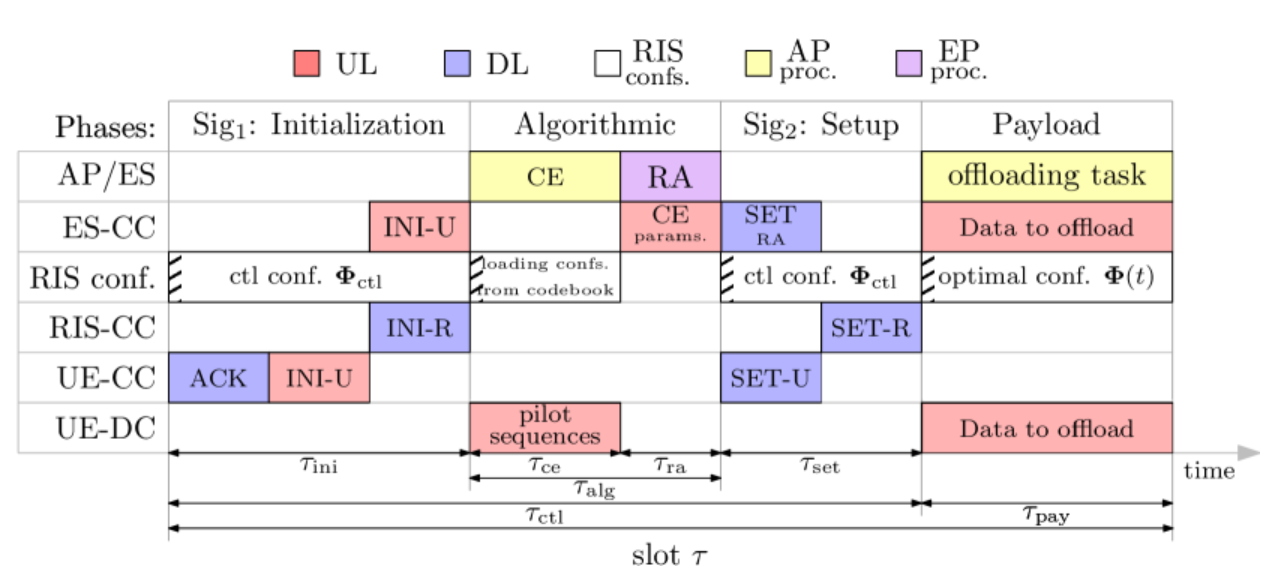
\includegraphics[width=1\textwidth]{images/f2.png}
  \caption{Sơ đồ thời gian một slot $t$. }
    \label{fig:my-image}
\end{figure}


Pha (a) Khởi tạo (Initialization): Mở đầu mỗi slot, AP và UE thực hiện thủ tục đồng bộ và chuẩn bị thông tin ban đầu. Cụ thể, AP gửi các bản tin ACK/NACK tới từng UE (thông báo UE biết dữ liệu gửi ở slot trước có nhận thành công không)
. Mỗi UE khi nhận NACK sẽ phải giữ lại dữ liệu chưa gửi thành công đó ở đầu hàng đợi để gửi lại, còn ACK thì có thể gỡ dữ liệu đã gửi ra khỏi hàng đợi
. Sau đó, mỗi UE gửi một gói điều khiển INI-U (Initialization-UE) lên AP thông qua kênh UE-CC UL, mang thông tin trạng thái hàng đợi của UE (ví dụ độ dài hàng đợi còn lại)
. AP thu thập các INI-U từ các UE và chuyển tiếp thông tin này tới ES qua kênh ES-CC
. Đồng thời, AP cũng gửi một gói INI-R (Initialization-RIS) tới RIS qua kênh RIS-CC để báo RIS chuẩn bị thực hiện ước lượng kênh
\cite{ris_latency}
. Cụ thể, lệnh INI-R yêu cầu RIS chuyển sang cấu hình điều khiển “ctl” – cấu hình pha đặc biệt có búp sóng rộng để phục vụ cho quá trình pilot (sẽ nói ở pha b)
. Trước khi RIS đổi sang cấu hình mới, cần một khoảng thời gian bảo vệ (guard period) do hạn chế phần cứng (ví dụ RIS cần vài micro-giây để thiết lập pha)
. Pha Initialization do đó bao gồm: thời gian phát các gói ACK (có thể đồng thời tới nhiều UE), thời gian UE gửi INI-U (có thể đồng thời nếu khác tần số do FDM), thời gian AP gửi INI-R (1 gói đơn), và thời gian guard chuyển cấu hình RIS. Công thức

\begin{equation}\label{eq:tau_ini}
\tau_{\mathrm{ini}} = \tau_{s} + 3T.
\end{equation}

mô tả tổng overhead thời gian cho pha Initialization $\tau_\text{ini}$, bao gồm các thành phần như trên
. Như vậy, $\tau_\text{ini}$ tỉ lệ với thời lượng gói điều khiển và thường khá nhỏ (vài TTI) nhưng không thể bỏ qua.


Pha (b) Thuật toán (Algorithmic): Đây là phần chính yếu của overhead, gồm hai quy trình: ước lượng kênh (CE) và tính toán phân bổ tài nguyên (RA).
\begin{itemize}
    \item Ước lượng kênh (CE): Nhằm biết được thông tin kênh CSI để tối ưu cấu hình, trong mỗi slot hệ thống phải dành thời gian cho UE gửi tín hiệu pilot. Với RIS, việc ước lượng phức tạp hơn do phải ước lượng cả kênh trực tiếp UE–AP lẫn kênh phản xạ qua RIS. Phương pháp phổ biến là sử dụng một bộ cấu hình RIS thử nghiệm (CE codebook) gồm $Q$ cấu hình khác nhau, lần lượt thiết lập RIS qua từng đợt pilot, để thu được $Q$ tín hiệu phản xạ, từ đó suy ra các thành phần kênh tương ứng
\cite{ris_latency}
. Cụ thể, trong bài báo, giả sử mỗi UE gửi một chuỗi pilot có độ dài $L$ TTI để ước lượng kênh trực tiếp (trong khi RIS tắt hoặc ở trạng thái mặc định), sau đó RIS lần lượt áp $Q$ cấu hình khác nhau và UE lặp lại chuỗi pilot $L$ TTI cho mỗi cấu hình. AP sẽ thu được $Q+1$ tín hiệu để tính ra kênh trực tiếp $h_{d}$ và $Q$ kết hợp $h_r$ tương ứng, từ đó suy luận kênh RIS–AP và UE–RIS riêng biệt
. Quá trình này diễn ra đồng thời cho tất cả UE (do FDM, mỗi UE ở băng riêng nên không nhiễu nhau)
. Giả sử $N$ phần tử RIS và kỹ thuật ước lượng cho phép nhóm các phần tử hoặc có độ suy giảm tự do, $Q$ có thể nhỏ hơn $N$ nhiều (các nghiên cứu CE cho RIS đề xuất $Q$ tỉ lệ $N$ hoặc $\log N$ tùy phương pháp
). Công thức cho thấy thời gian overhead CE là: $\tau_\text{CE} = L \cdot (1 + Q) + Q \cdot t_\text{switch}$
ar5iv.labs.arxiv.org
. Trong đó $t_\text{switch}$ là thời gian chuyển cấu hình RIS giữa các lần, nhân với $Q$ lần chuyển
. Rõ ràng, $\tau_\text{CE}$ tăng tỷ lệ với số cấu hình pilot $Q$. $Q$ càng lớn (kênh phức tạp, nhiều phần tử) thì overhead càng cao, bù lại CSI đầy đủ hơn. Nếu muốn giảm overhead, có thể giảm $Q$ nhưng khi đó thông tin kênh ít đi, có thể buộc hệ thống chấp nhận cấu hình RIS chưa tối ưu hoặc sử dụng thuật toán khác (như beam sweeping thay vì CE chính xác
).
    \item Tính toán phân bổ tài nguyên (RA): Sau khi có CSI (tạm coi đã có sau bước CE), máy chủ ES sẽ giải một bài toán tối ưu nhằm quyết định: cấu hình pha RIS tối ưu $\Phi^*(t)$ cho slot này, vector beamforming tại AP, phân bổ công suất cho mỗi UE, tần số CPU phục vụ mỗi UE, v.v., thỏa mãn các ràng buộc (như giới hạn năng lượng, đảm bảo trễ) và tối ưu hóa mục tiêu (như trễ trung bình nhỏ nhất hoặc năng lượng tiêu thụ tổng nhỏ nhất). Bài toán này thường phi tuyến và phức tạp, nhưng có thể giải bằng các thuật toán gần đúng (heuristic) hoặc tối ưu lồi hóa. Thuật toán được thực thi tại ES (hoặc AP) trong mỗi slot, do đó tiêu tốn thời gian tính toán – cũng chính là một phần overhead. Ký hiệu $\tau_\text{RA}$ là thời lượng ES/AP cần để hoàn tất thuật toán RA. Công thức (19) liên hệ $\tau_\text{RA} = \frac{C_\text{RA}}{f_\text{ES}}$ chẳng hạn, với $C_\text{RA}$ là số chu kỳ CPU cần để giải bài toán RA và $f_\text{ES}$ là xung nhịp CPU ES (chu kỳ/s) . Nếu ES dành một phần năng lực CPU cho RA song song với xử lý tác vụ thì có thể phức tạp; ở đây ta coi RA được ưu tiên làm trước rồi mới xử lý tác vụ. Từ giải thuật cụ thể, tác giả ước tính $C_\text{RA}$. Chẳng hạn, họ dùng thuật toán tham lam để tìm cấu hình RIS và beamforming AP tối ưu: cố định một vector beam tại AP, sau đó chọn dần cấu hình pha từng nhóm phần tử RIS sao cho cải thiện mục tiêu nhiều nhất . Số lựa chọn có thể duyệt cho một nhóm $g$ phần tử là $2 \times (2^b)^g$ (mỗi phần tử có 2 trạng thái: hoạt động hoặc tắt, và nếu hoạt động thì có $2^b$ mức pha lượng tử với $b$ bit phân giải) . Thuật toán lặp qua nhiều nhóm cho đến khi xét đủ $N$ phần tử hoặc đạt ngưỡng. Nếu chọn nhóm $g$ lớn (tức tối ưu theo cụm phần tử), độ phức tạp giảm nhưng hiệu quả giảm; nhóm $g=1$ (tối ưu từng phần tử) cho hiệu năng cao nhất nhưng phức tạp nhất . Cuối cùng, (20) đưa công thức tính số chu kỳ cần thiết $C_\text{RA}$ dựa trên số phép nhân phải thực hiện khi thử các khả năng . Kết luận: $\tau_\text{RA}$ càng lớn nếu bài toán phức tạp (nhiều biến như nhiều phần tử RIS) hoặc CPU chậm. Do đó, overhead điều khiển có thể giảm bằng cách giảm độ tối ưu (ví dụ nhóm nhiều phần tử RIS để giảm vòng lặp tính toán, chấp nhận cấu hình sub-optimal) .
\end{itemize}

Tổng thời gian pha Algorithmic là $\tau_\text{alg} = \tau_\text{CE} + \tau_\text{RA}$. Đây thường là phần chiếm nhiều nhất trong $\tau$.

Pha (c) Thiết lập (Setup): Sau khi ES tính toán xong các tham số tối ưu (công suất, tốc độ mã hóa, cấu hình RIS,...), AP sẽ gửi các thông tin thiết lập này trở lại UE và RIS để áp dụng trong phần truyền data của slot hiện tại  . Cụ thể, AP gửi gói SET-U cho từng UE chứa các tham số như: hệ số công suất $p_k(t)$ mà UE nên dùng, tốc độ dữ liệu (hoặc MCS – modulation and coding scheme) tối đa UE được phép truyền (dựa theo kênh ước lượng)  . Gói SET-U có thể gửi đồng loạt (broadcast hoặc multicast) nếu gọn, hoặc lần lượt nếu trễ cho phép. Đồng thời, AP gửi gói SET-R cho RIS chứa cấu hình pha tối ưu $\Phi^*(t)$ cần thiết lập  . Trước khi gửi SET-R, AP yêu cầu RIS chuyển sang chế độ nhận lệnh (thường RIS phải tạm thời về cấu hình “ctl” để dễ nhận tín hiệu điều khiển) – do đó cũng cần một khoảng guard ngắn để RIS chuyển trạng thái như ban đầu  . Tổng thời gian pha Setup $\tau_\text{setup}$ gồm thời gian phát các gói SET-U (có thể đồng thời trên nhiều tần số) + thời gian phát 1 gói SET-R + guard chuyển RIS về chế độ nhận lệnh. Công thức $\tau_\text{setup}$ gồm các thành phần đó.\cite{ris_latency}


Sau khi pha c) kết thúc, RIS có cấu hình mới $\Phi^*(t)$, các UE biết mình sẽ truyền bao nhiêu với công suất bao nhiêu, AP/ES sẵn sàng thu và xử lý – hệ thống chuyển sang pha (d) truyền dữ liệu (Payload) trong thời gian $T-\tau$. Tại đây, mỗi UE gửi một phần dữ liệu (có thể là toàn bộ hàng đợi nếu đủ thời gian) qua kênh UL. Nhờ có RIS điều chỉnh tối ưu và AP biết trước công suất truyền, việc tiếp nhận sẽ hiệu quả. AP thu tín hiệu, gỡ lỗi; cuối slot AP chuyển dữ liệu thu được sang ES xử lý (có thể xử lý song song để giảm độ trễ). Vòng lặp tiếp tục cho slot tiếp theo.


Tóm lại, overhead $\tau$ mỗi slot gồm 3 pha: Khởi tạo, Thuật toán, Thiết lập. Overhead này không cố định mà phụ thuộc vào tham số hệ thống và thiết kế giao thức: số UE, độ dài gói điều khiển, số cấu hình pilot $Q$, độ phức tạp thuật toán RA, tốc độ phần cứng (RIS switching, CPU), v.v. Bảng 1 (giả định) tóm tắt đóng góp của từng yếu tố vào $\tau$. Chẳng hạn, nếu muốn giảm độ trễ, ta có thể giảm $Q$ (nhưng đánh đổi độ chính xác CSI), hoặc dùng thuật toán RA đơn giản hơn (đánh đổi hiệu năng). Phần sau chúng tôi sẽ phân tích kỹ sự đánh đổi này.

\section{Overhead thời gian tác động đến độ trễ offload}


Overhead điều khiển lớn sẽ làm giảm thời gian payload mỗi slot, do đó nếu dữ liệu UE cần gửi nhiều, có thể không gửi kịp trong một slot, phải đợi slot sau -> tăng độ trễ hàng đợi. Ngược lại, overhead nhỏ giúp truyền được nhiều dữ liệu hơn mỗi slot, giảm hàng đợi, nhưng có thể khiến quyết định kém tối ưu gây giảm thông lượng hữu ích hoặc tăng lỗi gói. Có một điểm thú vị: nếu slot kéo dài hơn (T tăng) thì dù overhead $\tau$ có thể tăng theo nhưng tỷ lệ $\tau/T$ có thể giảm, tức hiệu suất truyền net cao hơn. Tuy nhiên, slot dài có nghĩa chu kỳ ra quyết định chậm, UE có thể phải chờ lâu để bắt đầu truyền -> không tốt cho trễ cá thể. Do đó, tồn tại một giá trị slot tối ưu cân bằng giữa hiệu suất và độ trễ.


Kết quả mô phỏng từ bài báo gốc (Hình 3) cho thấy hiệu năng hệ thống phụ thuộc mạnh vào độ dài slot $T$ (tương ứng tỷ lệ overhead). Cụ thể, Figure 3 vẽ tiêu thụ năng lượng trung bình, công suất trung bình mỗi slot, và độ trễ trung bình khi thay đổi $T$ trong trường hợp không có lỗi điều khiển .

\begin{figure}[H]
  \centering
  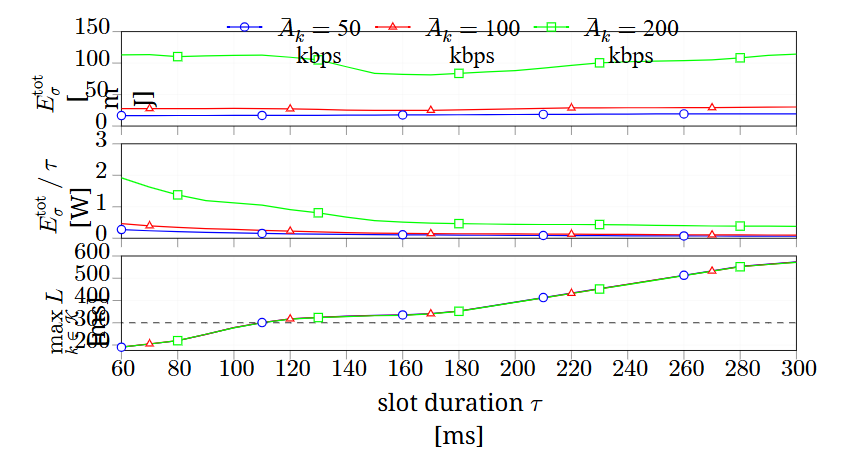
\includegraphics[width=0.8\textwidth]{images/f3.png}
  \caption{hiệu năng hệ thống phụ thuộc mạnh vào độ dài slot}
    \label{fig:my-image}
\end{figure}

Các đường tương ứng với các lưu lượng đầu vào khác nhau (50, 100, 200 kbps). Kết quả chỉ ra rằng có một khoảng $T$ tối ưu giúp tối thiểu hóa năng lượng tiêu thụ, đồng thời giữ trễ trong giới hạn. Nếu $T$ quá nhỏ (quá nhiều slot trong 1 giây), overhead tốn phần lớn thời gian -> mỗi slot truyền rất ít dữ liệu, UE phải tăng công suất để gửi kịp dẫn đến năng lượng cao và trễ hàng đợi tăng do nhiều slot mới xong dữ liệu . Nếu $T$ quá lớn, overhead tuy chiếm tỷ lệ nhỏ nhưng UE phải đợi lâu mới tới lần truyền: trong thời gian chờ, hàng đợi tích lũy gây trễ cao, đồng thời do ra quyết định thưa, có thể cấu hình RIS không kịp thích ứng kênh thay đổi. Mô phỏng cho thấy có $T$ tối ưu cỡ vài ms (tuỳ kịch bản) để đạt cực tiểu năng lượng tiêu thụ mà vẫn đảm bảo trễ thấp .


Một hệ quả khác: overhead nhiều nhất là do ước lượng kênh. Nếu kênh thay đổi chậm, ta không cần ước lượng lại quá thường xuyên. Ý tưởng điều khiển hai thang thời gian (two-timescale): RIS giữ cấu hình trong nhiều slot (chỉ update khi cần), còn data vẫn truyền mỗi slot. Như vậy overhead CE chia đều ra nhiều slot, giảm tỷ lệ $\tau/T$. Cách này hiệu quả khi kênh có tính bền (correlation cao qua thời gian). Một số nghiên cứu đã đề xuất ước lượng kênh two-timescale hoặc dựa vào học máy để giảm tần suất pilot. Tất nhiên, đánh đổi là cấu hình RIS không cập nhật kịp nếu kênh đổi đột ngột.


Từ góc nhìn hệ thống, overhead điều khiển làm giảm thông lượng khả dụng. Ta có thể hiệu chỉnh lại công thức tốc độ: nếu kênh capacity là $R$ (bit/s), thì tốc độ offload thực tế xem xét overhead là $R_\text{eff} = R \cdot \frac{T-\tau}{T}$ (bit/s). Tỷ lệ $\frac{T-\tau}{T}$ chính là hiệu suất sử dụng frame. Giả sử $\tau$ tỉ lệ tuyến tính với số phần tử RIS (trong ước lượng) hoặc độ phức tạp RA, khi hệ thống mở rộng (nhiều UE, RIS lớn) mà không cải tiến giao thức, overhead sẽ lấn át payload. Vì vậy, trong thiết kế MEC/RIS cần tìm cách hạn chế độ phức tạp tăng tuyến tính. Một ví dụ, thay vì tối ưu toàn bộ $N$ phần tử RIS, người ta có thể chia RIS thành các nhóm phần tử cố định (một nhóm điều khiển như một unit). Khi đó số biến cần tối ưu giảm, overhead CE và RA giảm, nhưng cái giá là giảm bớt độ tự do của RIS nên hiệu năng có thể kém hơn chút . Đây chính là một sự đánh đổi hiệu năng – overhead: cấu hình RIS càng linh hoạt (mỗi phần tử riêng biệt) thì càng tốn overhead; ép RIS gộp nhóm giảm overhead nhưng hiệu quả beamforming kém tối ưu hơn.


\section{Ảnh hưởng của overhead điều khiển đến tiêu thụ năng lượng}

Overhead thời gian không chỉ ảnh hưởng trễ mà còn liên quan chặt chẽ đến năng lượng tiêu thụ .


Thứ nhất, overhead càng lớn đồng nghĩa thiết bị và mạng phải hoạt động nhiều hơn cho việc điều khiển. Ví dụ, thời gian pilot dài hơn nghĩa là UE phát sóng liên tục lâu hơn, tiêu tốn nhiều năng lượng pin hơn . AP cũng phải phát nhiều tín hiệu điều khiển hơn, RIS duy trì hoạt động lâu hơn. Nếu overhead giảm, các thành phần có thể “nghỉ” sớm hơn để tiết kiệm năng lượng (tất nhiên phải cân bằng với hiệu năng).


Thứ hai, overhead cao làm giảm thời gian truyền data, để gửi cùng lượng data trong ít thời gian hơn, UE có thể phải dùng công suất phát cao hơn. Công suất phát tăng làm tiêu hao năng lượng pin phi tuyến (công suất cao làm hiệu suất khuếch đại kém đi). Đồng thời, công suất phát cao hơn dễ gây nhiễu liên cell hơn (nếu có tái sử dụng tần số), gián tiếp ảnh hưởng năng lượng toàn mạng. Trong Fig.3, khi slot quá nhỏ (overhead chiếm nhiều), người ta quan sát công suất trung bình tăng và do đó năng lượng mỗi bit tăng.


Thứ ba, overhead gồm phần tính toán thuật toán RA trên ES. Nếu thuật toán quá phức tạp, CPU ES phải chạy tần số cao (tăng $f$), theo công thức CMOS $E \propto f^2$, năng lượng ES tăng đáng kể . Năng lượng này dù không ảnh hưởng trực tiếp pin UE nhưng lại góp phần tiêu thụ điện của hạ tầng. Trong bối cảnh xanh hóa 6G, ta cũng cần giảm phần này. Vậy nên có quan điểm “tối ưu vừa đủ”: đôi khi giải một bài toán RA quá chính xác (tối ưu cận biên) không đáng, vì lợi ích năng lượng thu được nhỏ hơn năng lượng chính việc tính toán tiêu tốn.


Bài báo gốc cũng xem xét năng lượng cho RA như một phần của hàm mục tiêu. Hệ số trọng số $w$ cho phép cân nhắc giữa việc giảm năng lượng UE (liên quan overhead pilot, công suất) và giảm năng lượng mạng (liên quan overhead tính toán, AP, RIS)  . Trong nhiều trường hợp, giảm năng lượng UE được ưu tiên hơn (vì UE hạn chế pin), do đó có thể chấp nhận tốn năng lượng mạng (vốn cấp nguồn tốt) để giảm tải cho UE. Ví dụ, AP/ES có thể tăng overhead tính toán (dùng CPU mạnh tính nhanh RA) để tìm cấu hình giúp UE truyền ít tốn pin nhất (thời gian truyền ngắn, công suất thấp) – đây là cách hy sinh năng lượng mạng đổi lấy năng lượng UE . Ngược lại, nếu mạng muốn tiết kiệm điện (ví dụ trạm 5G dùng pin năng lượng mặt trời), có thể giảm tần suất RA, chấp nhận UE tốn pin hơn chút, miễn sao duy trì QoS.

Tóm lại, overhead điều khiển ảnh hưởng hai mặt: độ trễ và năng lượng. Thiết kế hệ thống MEC/RIS cần đặt mục tiêu tối ưu tổng thể, không chỉ tối đa tốc độ offload mà phải xét chi phí điều khiển đi kèm. Phần sau, chúng tôi sẽ đi sâu vào khía cạnh độ tin cậy: nếu overhead đã tối ưu mà kênh điều khiển lại gây lỗi, hiệu quả hệ thống sẽ ra sao.

\chapter{Đánh đổi hiệu năng và độ trễ dưới tác động của overhead}
Như phân tích ở trên, việc tăng/giảm overhead điều khiển dẫn đến đánh đổi (trade-off) giữa hiệu năng đạt được (thông lượng, năng lượng) và độ trễ. Trong phần này, chúng tôi tổng hợp một số góc nhìn về sự đánh đổi này dựa trên kết quả mô phỏng cũng như lý thuyết.


\section{Hiệu năng hệ thống theo tỷ lệ overhead điều khiển}

Hiệu năng thông lượng vs. overhead: Nếu bỏ qua lỗi, khi tăng overhead (thêm thời gian cho CE, RA), hệ thống đạt cấu hình gần tối ưu hơn, do đó thông lượng dữ liệu mỗi slot tăng (nhờ CSI chính xác, RIS tối ưu). Tuy nhiên, do thời gian truyền dữ liệu bị rút ngắn, nên lượng dữ liệu thực sự truyền được có thể không tăng tương ứng. Có điểm tới hạn: khi overhead vượt quá mức, thông lượng net giảm. Mô phỏng đã khẳng định có một tỷ lệ overhead tối ưu (khoảng 10-20pt tùy kịch bản) để tối đa hóa throughput net. Hiệu năng năng lượng vs. overhead: Một mặt, overhead cao giúp giảm năng lượng phát (vì cấu hình tốt, ít lãng phí công suất), nhưng mặt khác overhead chính nó tiêu tốn năng lượng (pilot dài, tính toán nhiều). Tổng năng lượng (UE+mạng) thường có điểm tối ưu tại overhead vừa phải. Kết quả từ Fig.3 (error-free) cho thấy năng lượng trung bình hệ thống thấp nhất tại một độ dài slot nhất định (tương ứng overhead ~15).


Khi overhead tăng hơn mức này, lợi ích giảm nhiêu liệu (vì UE có thể giảm công suất) không đủ bù đắp năng lượng phần điều khiển. Hiệu năng độ trễ vs. overhead: Overhead quá ít có thể gây thông lượng thấp do cấu hình xấu, khi đó hàng đợi kéo dài, tăng trễ. Overhead quá nhiều thì trực tiếp giảm thời gian phục vụ dữ liệu, trễ cũng tăng. Do đó, về độ trễ, cũng có mức overhead tối ưu. Thông thường, mức overhead tối ưu về trễ tương đồng với tối ưu năng lượng, vì trễ thấp thường đạt được khi hiệu quả năng lượng tốt (không lãng phí thời gian, không backlog). Một khía cạnh nữa: overhead tối ưu còn phụ thuộc mục tiêu QoS cụ thể. Nếu mục tiêu là độ trễ cực thấp (URLLC), ta có thể chấp nhận tốn năng lượng hơn miễn sao trễ giảm – tức sẵn sàng overhead nhiều để chắc chắn không mất gói, không phải truyền lại. Ngược lại nếu mục tiêu tiết kiệm năng lượng tối đa, có thể chịu trễ nhỉnh hơn chút, overhead có thể giảm.
\section{Chi phí năng lượng của các hoạt động điều khiển}

\begin{itemize}
    \item Năng lượng cho ước lượng kênh: tỉ lệ với độ dài pilot $L$ và số cấu hình $Q$. UE tiêu thụ $P_\text{UE}^\text{pilot} \cdot L (1+Q)$ (công suất pilot nhân thời gian) , RIS tiêu thụ $N P_\text{ele}$ trong thời gian đó . Nếu $Q$ lớn (RIS nhiều phần tử), đây là phần không nhỏ. Ví dụ, nếu mỗi pilot dùng 0.1 W, $L=1$ ms, $Q=50$ cấu hình, mỗi UE dùng 0.1*0.051=0.0051 J cho pilot mỗi slot, ước tính ~5 mJ. Với 10 UE, ~50 mJ, khá đáng kể nếu slot ngắn. Giảm $Q$ sẽ cắt giảm gần tỉ lệ.
    \item Năng lượng cho tính toán RA: $E^\text{ES}\text{ctl} = C\text{RA} \cdot C (f_\text{ES})^2$ (coi CPU ES hoạt động ở điện áp cho trước). Nếu thuật toán phức tạp gấp đôi, $C_\text{RA}$ tăng gấp đôi, năng lượng tăng đôi. Tuy không trực tiếp ảnh hưởng UE, nhưng trong viễn cảnh MEC dùng server chạy bằng pin (như MEC di động gắn UAV) thì rất quan trọng.
    \item Năng lượng cho signaling: AP phát ACK, SET-U, SET-R... thường công suất nhỏ (control channel công suất thấp hơn data). Nhưng nếu nhiều gói và dài, tổng cũng không bỏ qua được. RIS controller có thể tiêu thụ cỡ vài mW cho mỗi lần nhận lệnh.
\end{itemize}


Những chi phí này có thể ẩn khi đánh giá, nhưng để thiết kế tối ưu cần đưa chúng vào hàm mục tiêu. Một số nghiên cứu khác cũng đề cập việc định lượng chi phí tín hiệu điều khiển. Ví dụ, Anders Enqvist và cs. (2025) phân tích số bit tín hiệu phản hồi cần thiết cho RIS và ảnh hưởng của nó đến SNR, đề xuất mã hóa lượng tử hóa để giảm overhead điều khiển trong khi chỉ giảm SNR chút ít. Các hướng như vậy đều nhằm giảm năng lượng phần điều khiển mà vẫn duy trì hiệu năng cao.
\section{Tối ưu hóa phân bổ tài nguyên vs. chi phí tính toán (RA algorithm)}

Nói riêng về thuật toán RA, đây là thành phần đặc trưng của MEC/RIS. Thuật toán RA quyết định hiệu năng nhưng đồng thời tạo overhead tính toán. Do đó có sự đánh đổi giữa:

\begin{itemize}
    \item Thuật toán chính xác cao (optimal): đạt hiệu năng tối đa (ví dụ thông lượng cao nhất, năng lượng tiêu thụ ít nhất), nhưng thời gian chạy dài, có thể vượt quá slot nếu không cẩn thận, hoặc tiêu hao nhiều CPU -> không phù hợp thời gian thực.
    \item Thuật toán xấp xỉ/heuristic nhanh: cho kết quả gần tối ưu, chạy nhanh (vài ms), overhead nhỏ, nhưng hiệu năng có thể thấp hơn ngưỡng yêu cầu.
\end{itemize}

Lựa chọn thuật toán tùy thuộc mục tiêu hệ thống: nếu yêu cầu độ trễ nghiêm ngặt và hệ thống thay đổi nhanh, cần thuật toán rất nhanh, chấp nhận suboptimal. Ngược lại nếu kênh ít thay đổi và cần vắt kiệt hiệu năng, có thể chạy thuật toán kỹ hơn.

Bài báo gốc chọn thuật toán tham lam (greedy) để giảm độ phức tạp . Họ cũng giới hạn việc tối ưu RIS theo nhóm thay vì từng phần tử để giảm $C_\text{RA}$ . Kết quả, overhead RA (tính bằng ms) giảm nhiều so với nếu thử hết $2^{Nb}$ khả năng.

Một xu hướng mới là dùng học máy/học sâu để làm RA: mạng neural có thể được huấn luyện để gần như trực tiếp dự đoán cấu hình tối ưu từ CSI, thay vì giải tối ưu lặp. Điều này có thể giảm thời gian tính toán khi triển khai (suy luận mạng neural rất nhanh trên GPU), nhưng đánh đổi là cần dữ liệu huấn luyện và có sai số. Tuy nhiên, nếu sai số nhỏ chấp nhận được, đây là cách giảm overhead RA rất hứa hẹn. Một số nghiên cứu RIS gợi ý hướng này.


\chapter{Tác động của lỗi điều khiển và độ tin cậy kênh điều khiển}
Trong các phần trước, chúng tôi giả định ngầm rằng các tín hiệu điều khiển (pilot, gói INI, SET...) được trao đổi thành công 100 phần trăm và kênh ước lượng chính xác. Thực tế, kênh điều khiển cũng chịu lỗi (nhiễu, fading) và quá trình ước lượng kênh có sai số. Những lỗi điều khiển này sẽ ảnh hưởng trực tiếp đến các quyết định trong hệ thống MEC/RIS, nếu không được tính đến thì hiệu năng thực tế có thể kém xa so với tính toán lý thuyết.


\section{Lỗi ước lượng kênh (CE) và hệ quả đến thông lượng}

Ước lượng kênh sai (CSI error) xảy ra do pilot nhiễu, do mô hình chưa đủ, hoặc do thời gian giữa pilot và truyền data kênh đã đổi (quá hạn). Lỗi CSI nghĩa là AP và ES không biết chính xác gain kênh. Khi đó, quyết định RA có thể không phù hợp thực tế: ví dụ, giả sử AP nghĩ kênh UE tốt hơn thực tế → ES sẽ đặt tốc độ truyền quá cao (MCS quá lớn) cho UE, hoặc giảm công suất UE vì nghĩ không cần cao -> kết quả UE truyền không đạt throughput yêu cầu, có thể mất một phần hoặc toàn bộ gói data (giải mã thất bại do chọn MCS vượt SNR thực). Ngược lại, nếu AP đánh giá kênh xấu hơn thực → ES có thể cho MCS quá thận trọng hoặc công suất quá cao -> lãng phí tài nguyên và năng lượng, mặc dù dữ liệu vẫn tới đích.


Trường hợp xấu nhất của lỗi CE: UE truyền với tốc độ danh định cao hơn dung lượng kênh thực, dẫn đến toàn bộ gói payload mất trong slot đó. Điều này tương đương trễ tăng thêm một slot (phải chờ retransmit) hoặc thậm chí mất gói nếu không có HARQ. Bài báo định nghĩa thông lượng danh định theo CSI ước lượng (công thức (14)), và thông lượng thực tế giảm khi có lỗi CE khiến danh định vượt quá capacity . Từ Proposition 1, nếu dùng phương pháp ước lượng Least Squares (LS) với pilot lặp $L$ lần, trong kênh Rayleigh, phương sai lỗi ước lượng có thể tính được: nó tỉ lệ nghịch với $L$ (pilot dài hơn -> lỗi nhỏ)  . Do đó, một cách giảm lỗi CE là tăng độ dài pilot hoặc công suất pilot, nhưng lại tăng overhead.


Thay vì tăng pilot, cũng có thể dùng thuật toán ước lượng tốt hơn (MMSE, Bayesian) nếu có thông tin prior, giúp giảm lỗi ở cùng $L$. Tuy nhiên, dù sao sai số khác 0 vẫn tồn tại. Hướng khác: thiết kế RA robust với lỗi CSI – tức thay vì tối ưu dựa trên CSI ước lượng như thật, ES có thể tối ưu theo kiểu "worst-case" hoặc "đặt margin" cho an toàn. Ví dụ, nếu kênh ước lượng SNR = 20 dB, ES có thể chọn MCS ứng với 15 dB thôi để dằn sai số. Cách này giảm rủi ro mất gói do CSI sai, nhưng đánh đổi throughput khi CSI đúng.

Tóm lại, lỗi CE có thể làm giảm thông lượng thực so với tính toán, thậm chí làm mất ổn định hàng đợi nếu hệ thống không phát hiện để bù đắp. Vì vậy, các giải pháp MEC/RIS cần kết hợp kỹ thuật kiểm soát lỗi – ví dụ ARQ/HARQ để phục hồi khi gói payload mất do CSI sai.

\section{Mất gói tin điều khiển và ảnh hưởng tới quyết định hệ thống}
Có 4 loại gói control quan trọng trong giao thức: INI-U, INI-R, SET-U, SET-R (ngoài ra ACK nữa nhưng như bài báo lưu ý, ACK được giả định luôn truyền thành công nhờ bảo mật nội dung ngắn, ta bỏ qua). Xét từng trường hợp mất gói:

\begin{itemize}
    \item Mất gói INI-U (UE -> AP): Gói này mang thông tin trạng thái hàng đợi của UE gửi lên ES trước khi RA. Nếu mất, ES không biết lượng dữ liệu mới UE có. Bài báo giả định ES sẽ suy luận dựa trên dữ liệu đã nhận: nếu gói INI-U mất, ES tạm giả sử hàng đợi UE không có dữ liệu mới ngoài cái đã gửi ở slot trước . Điều này có thể sai nếu trong thời gian qua có thêm dữ liệu. Hệ quả: RA có thể cấp tài nguyên ít hơn cần thiết cho UE đó (vì tưởng UE gần hết data), dẫn đến trễ tăng do phần dữ liệu mới không được offload kịp. Tuy nhiên, vì RA còn tối ưu chung, UE này có thể bị thiệt thòi. Giải pháp: có thể thiết kế UE tự gửi lại INI-U nếu không nhận được phản hồi trong thời gian (nhưng phức tạp) hoặc dự đoán lượng đến.
    \item Mất gói INI-R (AP -> RIS): Gói này ra lệnh RIS chuyển sang chế độ ước lượng kênh (thay đổi cấu hình codebook). Nếu RIS không nhận được, nó sẽ không biết cần làm gì. Bài báo giả sử trường hợp xấu: RIS vẫn giữ cấu hình mặc định (ctl) trong suốt quá trình CE, nghĩa là AP chỉ nhận được pilot của kênh trực tiếp, không thu được gì từ kênh phản xạ . Về bản chất, CE phản xạ thất bại -> AP không có CSI về kênh qua RIS. Nếu không có chiến lược dự phòng, ES sẽ không thể tối ưu RIS (vì không biết kênh), có thể phải chọn config RIS ngẫu nhiên hoặc xấu nhất. Bài báo giả định trong trường hợp này, hệ thống không có CSI RIS nên đặt thông lượng danh định = 0 cho các UE qua RIS . Nói cách khác, coi như phiên offload thất bại hoàn toàn (vì không dám offload gì). Đây là tình huống nghiêm trọng nhất: mất 1 gói INI-R có thể làm lỡ toàn bộ slot cho nhiều UE. Do đó, gói INI-R cần được truyền thật tin cậy. Giải pháp: có thể dùng kênh out-of-band hoặc lặp lại gói; hoặc thiết kế nếu INI-R không ACK, AP \& RIS có mặc định an toàn (như luôn chạy quy trình beam sweeping thay vì tắt). Rõ ràng, kênh RIS-CC phải rất tin cậy để MEC/RIS vận hành tốt.
    \item Mất gói SET-U (AP -> UE): Gói này mang các tham số tối ưu (công suất, tốc độ) cho UE để UE truyền trong payload. Nếu UE không nhận được, nó không biết mình nên truyền thế nào. Bài báo giả định UE sẽ phải dùng lại cấu hình của slot trước (về công suất và tốc độ dữ liệu) và hy vọng AP giải mã được . Chiến lược này hợp lý: nếu kênh không thay đổi nhiều, dùng cấu hình cũ có thể vẫn ổn; nhưng nếu kênh đã thay đổi hoặc RA mới phân tài nguyên khác (ví dụ tăng rate), thì UE có thể đang dùng param lạc hậu. Trường hợp xấu: nếu lẽ ra RA muốn UE tăng công suất vì kênh xấu đi, mà UE vẫn phát yếu như slot trước, khả năng gói data này bị lỗi (do SNR không đủ cho MCS cũ). Hoặc ngược lại, RA giảm phân bổ cho UE (ví dụ ít băng thông hơn) mà UE vẫn gửi nhiều như trước -> tràn gói, xung đột. Bài báo đơn giản xét kịch bản: UE cứ phát như trước, AP cố giải mã, có thể lỗi tùy kênh  . Như vậy, mất SET-U thường ảnh hưởng cục bộ một UE, không làm hỏng toàn hệ nhưng gây giảm throughput và cần truyền lại. Giải pháp: AP có thể lắng nghe UL, nếu thấy UE dùng sai param có thể yêu cầu dừng (nhưng trong 1 slot ngắn khó kịp). Tốt hơn là nâng độ tin cậy UE-CC (mã hóa, lặp).
    \item Mất gói SET-R (AP -> RIS): Gói này mang cấu hình RIS tối ưu cho payload. Nếu RIS không nhận, nó sẽ không thể áp dụng cấu hình mới. Có thể RIS sẽ giữ nguyên cấu hình cũ từ slot trước (vì không có lệnh mới) hoặc tệ hơn, do ta đã chuyển sang control mode ở pha Setup, RIS có thể vẫn ở chế độ ctl rộng, không quay về cấu hình trước (tùy implement). Bài báo cho biết nếu SET-R mất, RIS chỉ có thể dùng lại $\Phi$ cũ (có thể hiểu là giữ cấu hình slot $t-1$ cho slot $t$). Nếu kênh không đổi nhiều, cấu hình cũ có thể vẫn ok, nhưng nếu UE di chuyển, config cũ có thể không tối ưu cho vị trí mới -> throughput giảm. Trường hợp xấu: nếu slot trước RIS để ctl config (giả sử slot trước bị lỗi CE), thì slot này cũng ctl config -> giống như không sử dụng RIS hiệu quả. Vậy mất SET-R cũng giống hệ thống bỏ lỡ lợi ích RIS trong slot hiện tại. Hậu quả có thể trên mọi UE nếu kênh direct xấu, throughput sụt. 
\end{itemize}


Tóm lại, trong các gói, INI-R và SET-R là quan trọng cho toàn hệ (vì ảnh hưởng chức năng RIS), SET-U quan trọng cho từng UE, INI-U tác động nhẹ nhất (ES có thể đoán). Fig.4 trong bài báo minh họa hiệu năng hệ thống theo xác suất lỗi gói điều khiển cho từng loại gói
ar5iv.org
. Kết quả chỉ ra, khi xác suất lỗi tăng, hiệu năng giảm mạnh, trong đó đường cong ứng với lỗi INI-R và SET-R suy giảm nặng nhất – khẳng định tầm quan trọng của chúng. Với xác suất lỗi control tầm $10^{-2}$ (1 phần trăm), độ trễ trung bình có thể tăng hàng chục phần trăm
. Điều này cho thấy MEC/RIS yêu cầu kênh điều khiển rất đáng tin cậy (tương đương URLLC).


Giải pháp tổng thể:
\begin{itemize}
    \item Dùng mã hóa kênh mạnh cho gói control (ví dụ mã LDPC dài, thấp tốc độ) để đảm bảo xác suất lỗi cực thấp, chấp nhận overhead tăng chút.
    \item Sử dụng công nghệ diversity: phát lặp lại gói điều khiển vài lần, hoặc gửi qua nhiều tần số/tuyến đường (nếu có).
    \item Thiết kế giao thức dự phòng: nếu phát hiện mất gói (ví dụ UE không nhận SET-U có thể báo NACK, AP re-send nhanh trong slot), hoặc fallback như trong trường hợp UE dùng cấu hình cũ, RIS giữ config cũ.
    \item Sử dụng kênh out-of-band cho RIS-CC, UE-CC trong ứng dụng đòi hỏi nghiêm ngặt, để tách biệt hẳn khỏi data, có thể điều chế robust hơn.
\end{itemize}
\section{Yêu cầu độ tin cậy cho kênh điều khiển trong ứng dụng độ trễ thấp}

Từ các phân tích trên, có thể thấy hệ MEC/RIS đặt ra yêu cầu khắt khe cho kênh điều khiển:

\begin{itemize}
    \item Độ trễ truyền gói điều khiển phải rất thấp: vì các pha signaling diễn ra nối tiếp trong slot, nếu gói điều khiển mất quá lâu (do ARQ nhiều lần) sẽ ảnh hưởng tiến độ. Do đó, thường chỉ cho phép 1-2 lần phát lại trong cùng slot, hoặc tốt hơn là thiết kế để hầu như không phải phát lại.
    \item Xác suất lỗi gói cực thấp: để network chạy trơn tru, có thể cần $P_e$ cho gói control cỡ $10^{-5}$ hoặc thấp hơn. Con số này tương tự yêu cầu URLLC (chẳng hạn 99.999pt reliability).
    \item Dung lượng kênh control phù hợp: gói control không lớn (vài byte đến vài chục byte), nhưng nếu nhiều UE thì tổng data control cũng đáng kể. Kênh UE-CC và RIS-CC phải có đủ băng thông để gửi hết gói trong khoảng thời gian nhỏ. Nếu in-band, cần hy sinh một phần băng thông data cho control.
\end{itemize}

Một ý tưởng hay: vì gói control nhỏ, có thể tận dụng kỹ thuật spread spectrum (trải phổ) để truyền chúng với mức lỗi cực thấp mà không ảnh hưởng nhiều đến data. Ví dụ trong 5G, PUCCH gửi điều khiển UL dùng mã với độ lợi lớn.


Đối với RIS, để giảm lỗi, người ta cũng có thể tích hợp cảm biến hoặc mạch thu trên RIS (gọi là RIS bán chủ động) để RIS có thể xác nhận lệnh nhận được – giống như thiết bị thu, thay vì hoàn toàn thụ động chờ tín hiệu đến đủ mạnh mới kích hoạt. Nhưng điều này tăng chi phí phần cứng.


Nhìn chung, giải pháp quan trọng nhất vẫn là thiết kế giao thức chịu lỗi: tức giả định sẽ có lúc gói control mất, hệ thống có khả năng tự vận hành an toàn ở chế độ degrade thay vì sập. Ví dụ: nếu CE không có (mất INI-R), có thể fallback sang chế độ beam sweeping mặc định trong slot đó (AP quét beam RIS theo codebook cố định, hy sinh hiệu suất nhưng tránh mất trắng dữ liệu). Hoặc nếu SET-R mất, RIS có thể tự động giữ cấu hình cũ chứ không reset ctl (như ta giả định trên). Tương tự, UE có thể đặt ngưỡng: nếu nó đo kênh thấy SNR thay đổi lớn mà không nhận SET-U, có thể tự tăng công suất để giảm nguy cơ mất gói.


Tóm lại, tính robust phải được đưa vào thiết kế MEC/RIS. Bài báo gốc đã tiên phong chỉ ra điều này, do đó mở ra hướng nghiên cứu tập trung vào giao thức và chiến lược điều khiển tin cậy trong mạng RIS, thay vì chỉ chăm chú lớp vật lý.

    

\chapter{Kết luận}
Báo cáo đã trình bày một cái nhìn toàn diện về các khía cạnh điều khiển trong hệ thống MEC được hỗ trợ bởi RIS, đặc biệt hướng tới ứng dụng yêu cầu độ trễ nghiêm ngặt. Từ việc phân tích mô hình, chúng tôi nhấn mạnh rằng bên cạnh những lợi ích rõ rệt do RIS mang lại (cải thiện chất lượng kênh, tăng tốc độ offload, giảm trễ truyền), thì chi phí và độ phức tạp của việc điều khiển RIS không thể bỏ qua trong thiết kế hệ thống :

\begin{itemize}
    \item Chi phí năng lượng: Việc sử dụng RIS không phải miễn phí về năng lượng – khi xem xét toàn hệ, năng lượng tiêu tốn bởi các quy trình điều khiển (phát pilot, xử lý thuật toán, tín hiệu điều khiển) và bởi bản thân thiết bị RIS (đặc biệt nếu là RIS chủ động) đóng góp đáng kể  . Một thiết kế hiệu quả cần cân bằng bài toán năng lượng giữa phía người dùng và phía mạng, ví dụ thông qua tham số trọng số $w$ trong hàm mục tiêu .
    \item Độ tin cậy của điều khiển: Chúng tôi đặc biệt lưu ý rằng kênh điều khiển phải được đảm bảo độ tin cậy cao trong các hệ thống MEC/RIS. Các lỗi trong ước lượng kênh và mất mát tín hiệu điều khiển (như lệnh cấu hình RIS, thông tin hàng đợi UE) đều có thể dẫn đến suy giảm nghiêm trọng chất lượng dịch vụ  . Do đó, bên cạnh việc tối ưu hiệu năng trung bình, hệ thống cần cơ chế dự phòng và thiết kế giao thức để chịu lỗi (fault-tolerant) trước các trục trặc control, nhằm giữ độ trễ trong giới hạn dù trong tình huống xấu.
    \item Thành phần overhead thời gian: Mỗi chu kỳ offload phải hy sinh một phần thời gian cho việc ước lượng kênh, tính toán tối ưu tài nguyên và trao đổi tín hiệu điều khiển. Tỷ lệ overhead này nếu không được tính tối ưu có thể lấn át lợi ích từ RIS, làm tăng độ trễ thay vì giảm  . Kết quả phân tích và mô phỏng cho thấy tồn tại một điểm cân bằng tối ưu về overhead giúp tối ưu hóa hiệu năng-tổng thể (thông lượng, năng lượng, trễ).
\end{itemize}



Tóm lại, việc tích hợp RIS vào MEC không chỉ là vấn đề tối ưu vật lý truyền dẫn, mà còn là một bài toán điều khiển liên tầng phức tạp, đòi hỏi cách tiếp cận toàn diện từ tầng vật lý đến tầng mạng. Những hiểu biết về overhead thời gian, chi phí năng lượng và độ tin cậy trình bày trong báo cáo này hy vọng sẽ giúp các kỹ sư và nhà nghiên cứu thiết kế các hệ thống MEC/RIS tương lai một cách thông minh hơn, đạt được hiệu quả cao mà vẫn đảm bảo được những yêu cầu QoS khắt khe của các ứng dụng thế hệ mới.
% \chapter*{Tài liệu tham khảo}
% \noindent [1] Shaka Player. https://shaka-player-demo.appspot.com/docs/api/index.html. Accessed: May 15, 2025.

\noindent [2] Adam, Giuseppe Samela. (2023). Adaptive Bitrate Streaming Evolved: WISH ABR and Bitmovin’s Player Integration. https://bitmovin.com/blog/wish-abr-adaptive-bitrate-streaming. Accessed: May 16, 2025.

\noindent [3] Vijaya Sagar Vinnakota. (2021). A TL;DR on ABR algorithms in MPEG DASH.
https://www.linkedin.com/pulse/tldr-abr-algorithms-mpeg-dash-vijaya-sagar-vinnakota. Accessed: May 17, 2025.

\noindent [4] Ziyu Zhong, Mufan Liu, Le Yang, Yifan Wang, Yiling Xu, Jenq-Neng Hwang. (2025). Video Streaming with Kairos: An MPC-Based ABR with Streaming-Aware Throughput Prediction. https://cs.paperswithcode.com/paper/video-streaming-with-kairos-an-mpc-based-abr. Accessed: May 19, 2025.

\noindent [5] Yueheng Li, Qianyuan Zheng, Zicheng Zhang, Hao Chen, Zhan Ma. (2025). Improving ABR Performance for Short Video Streaming Using
Multi-Agent Reinforcement Learning with Expert Guidance. https://arxiv.org/pdf/2304.04637. Accessed: May 22, 2025.

\noindent [6] Huang, Tianchi and Yao, Xin and Wu, Chenglei and Zhang, Rui-Xiao and Sun, Lifeng. (2018). Tiyuntsong: A Self-Play Reinforcement Learning Approach for ABR Video Streaming. https://github.com/thu-media/Tiyuntsong. Accessed: May 23, 2025.

\noindent [7] Lisa. What is WISH ABR? Revolutionizing Adaptive Streaming Quality.
https://www.coconut.co/articles/wish-abr-revolutionizing-adaptive-streaming-quality. Accessed: Jun 3, 2025.

\noindent [8] Version History of Shaka Player. https://github.com/shaka-project/shaka-player/releases?utm\_source=chatgpt.com. Accessed: Jun 4, 2025.



\printbibliography[heading=bibintoc]

\end{document}